\documentclass[a4paper,12pt]{article}
%\usepackage[ngerman]{babel}
\usepackage{ucs}
\usepackage{multirow}
\usepackage{xltxtra}
\usepackage[utf8x]{inputenc}
\usepackage{fontspec}
\usepackage[automark]{scrpage2}
\usepackage{eurosym}
\usepackage{graphicx}
\usepackage[paper=a4paper,left=25mm,right=25mm,top=25mm,bottom=25mm]{geometry}
\pagestyle{scrheadings}
\setmainfont[Mapping=tex-text]{Liberation Serif}
\clearscrheadfoot
\begin{document}
\ohead{Last edit: \today}
\title{Rules Linefollowing Challenge 2018}

 \begin{center}

\includegraphics[width=0.5\textwidth]{logo.png}

\huge                      % Schriftgröße einstellen
\bfseries                   % Fettdruck einschalten
Rules Linefollowing Challenge 2018
  \end{center}
   This is only an unofficial translation. In case of any doubt, only the newest official version of the German rules will
   count.
\section{Goal}
To design, build, and program a line following robot that can follow a black line on a white
background to a tower and deliver at first, at least one (1) ball and then return to its starting
point. Then in the remaining time (of 3 minutes) to return to the tower (as many times as
needed) to deliver a set number
(not over, not under) of balls as per their division’s
requirements.
\section{Who Can Play}
Teams of 2 to 4 players in separate divisions for:
\begin{itemize}
		\item Middle School (Age 10-13)
		\item High School (Age 14-17)
		\item Big Kids (Age 18-20)
\end{itemize}
\section{Required Materials}
Autonomous robot, any platform, costing \euro{1500}  or less, and meets the following design
constraints, which will be verified during Check-In:

\begin{itemize}
	\item Robot can demonstrate it is running a line following program by negotiating the final 60 cm of
	the current year's line following track (if an intersection is present within the last 60 cm, robot
	will start just past the intersection).
	\item Robot can demonstrate it will stop upon reaching the tower (you do not have to prove the ability
	to deliver a ball, or turn around).
	\item Volume of the robot must not
	exceed 65030 cubic cm. Multiple sensors and processors are
	allowed.
\end{itemize}
\section{General Rules of Play}
\begin{itemize}
	\item A line following program must control your robot’s motion.
	\item The robot has 3 minutes to complete the tasks.
	\item Only Players can operate and manipulate the robot during the heat. Remember: “Players Play,
	Coaches Coach”
	\item The tower
	cannot be touched by any person during the delivery.
	\item Touching the robot at any time requires it to be picked up and returned to home.
\end{itemize}
\section{Challenge Specifications}

\emph{The Track:}
\begin{itemize}
	\item White PVC Vinyl Background
	\item Middle School Division - One intersection, 1.3cm Black Line
	\item High School & Big Kid Division - Two intersections, 0.75cm Black Line
\end{itemize}
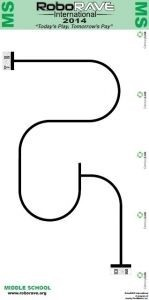
\includegraphics[width=0.3\textwidth]{track_ms_lf.png}
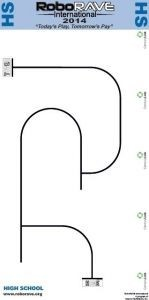
\includegraphics[width=0.3\textwidth]{track_hs_lf.png}

\emph{The Tower:}
\begin{itemize}
\item All divisions use the same – approximately 20cm tall, 10cm wide, and 35cm long with a 10cm x
10cm opening at the top and an open back to allow the balls to roll out during delivery. The
tower is held firm to the track by a strip of Velcro tape.
\item Using the same cardboard box tower/opening, we may attach or include a ramp or other
structure designed to count balls automatically as they flow through the tower. The design will
be such that it doesn’t impede the flow of balls through the tower, and may actually improve the
flow of balls.
\end{itemize}
\emph{The Competition Track and Tower Cannot be Modified for Any Reason!}
\section{Scoring Period}
\par The way the earned points are counted for the challenge will be announced on the first day of the event.
\section{Scoring}
The overall score is a combination of points earned to run the track to the tower, deliver at least
one ball, and then returning back home; and the number of required balls before the three
minutes runs out.
\begin{itemize}
\item Each division will have a set number of balls to deliver in the 3 minutes:
\begin{itemize}
	\item Middle School – 248
\item High School – 362
\item Big Kids - 437
\end{itemize}
\itemIf the number of balls is over
the required number of balls, the extra will be
subtracted
from the required number resulting in your ball score. If the number is fewer than the required
number, then that number is your ball score.
\item The 1st ball delivered is not counted as a ball but scored as the demonstration of being able
to deliver a ball to the tower. Only
than
one is not
1 ball
has to
be delivered! Delivering more
a penalty or a benefit - it is all scored as a demonstration of successful
delivery. The 1 ball (or more) are not counted as your required amount. They will be removed
before delivery of the required balls.
\item If you deliver the required number of balls before the 3 minutes has expired then stop!
See the Line Following score card for your division below for details on the scores assigned
during your first trip to the tower and back.
See the Line Following score card for your division below for details on the scores assigned
during your first trip to the tower and back.
\end{itemize}
\section{Scoring Matrix}
\begin{center}
\begin{tabular}{|c|c|c|c|c|c|} \hline
	\multirow{3}*{} & Leaves & Turns @ & Turns @ & Stops @ & Liefert einen \\
	 & Home & 1st “T” & 2nd “T” & Karton & Delivers \\ \hline
	MS & 25 & 25 & NA & 100 & 100 \\ \hline
	HS & 25 & 25 & 25 & 50 & 100 \\ \hline
	BK & 25 & 25 & 25 & 50 & 100 \\ \hline
\end{tabular}
\begin{tabular}{|c|c|c|c|c|c|} \hline
	\multirow{3}*{} & Starts Back & Turns @ & Turns @ & Returns & Total \\
	& Home & 1st “T” & 2nd “T” & Home &  \\ \hline
	MS & 25 & 25 & NA & 100 & 400 \\ \hline
	HS & 25 & 25 & 25 & 100 & 400 \\ \hline
	BK & 25 & 25 & 25 & 100 & 400 \\ \hline
\end{tabular}
\end{center}
\end{document}